Ce chapitre présente le problème rencontré par \cite{Vardhan04} et la technique générale utilisée pour proposer une solution à ce problème dans la section \ref{app}. Ce problème s'intéresse à la proriété de sûreté des automates à files définis dans le chapitre \ref{pre}. L'approche définie, un langage particulier est introduit : le langage de traces annotées de la section \ref{trace}. Celui-ci permet de représenter certains systèmes de transitions, infinis, par des langages régulier et donc des ADF. Utilisant une version modifiée de l'algorithme d'Angluin, les oracles d'appartenance et d'équivalence sont ajustés respectivement dans les sections \ref{mem} et \ref{eq}.

Finalement, la sûreté est définie formellement à la section \ref{safety}. Tous ces éléments mis ensemble permettent de compléter l'approche proposée dans la section \ref{app}. Les détails algorithmiques sont consignés dans le chapitre \ref{impl}.


\section{Approche}\label{app}Les automates à files définis à la section \ref{fifo} sont plus puissants que les ADF définis dans la section \ref{adf}. En effet, les systèmes de transitions associés ont potentiellement une infinité de configurations. Dans ces conditions, il n'est pas possible de faire une exploration exhaustive des états pour trouver lesquels sont acceptants.

À la place, une propriété dite de sécurité est définie. Si un état respecte cette propriété, il est \emph{sûr}. Si il y a moyen de prouver que la totalité des états de l'automate respectent cette propriété, l'automate est considéré comme sûr. Si au contraire, un exemple de violation de la propriété est trouvé, l'automate peut être déclaré comme à risque.

L'idée dès lors est de travailler non pas avec un système de transitions infini mais avec une représentation construite pour être finie dans un vaste ensemble de problèmes. Cette représentation est le langage de trace défini dans la section \ref{trace}.

En supposant que celui-ci est régulier, il est possible d'utiliser l'algorithme d'Angluin de la section \ref{angluin} pour l'apprendre. Cependant, ce langage n'est qu'un concept et le professeur n'a accès qu'à un automate à files $F$. Pour cette raison, les oracles d'appartenance et d'équivalence sont adaptés pour répondre à une requête entre un langage fourni par l'élève et $F$.

La figure \ref{fig:lever} donne une vue schématique de ce nouvel algorithme d'Angluin modifié.


\begin{figure}[H]
	\centering

	\resizebox{\textwidth}{!}{
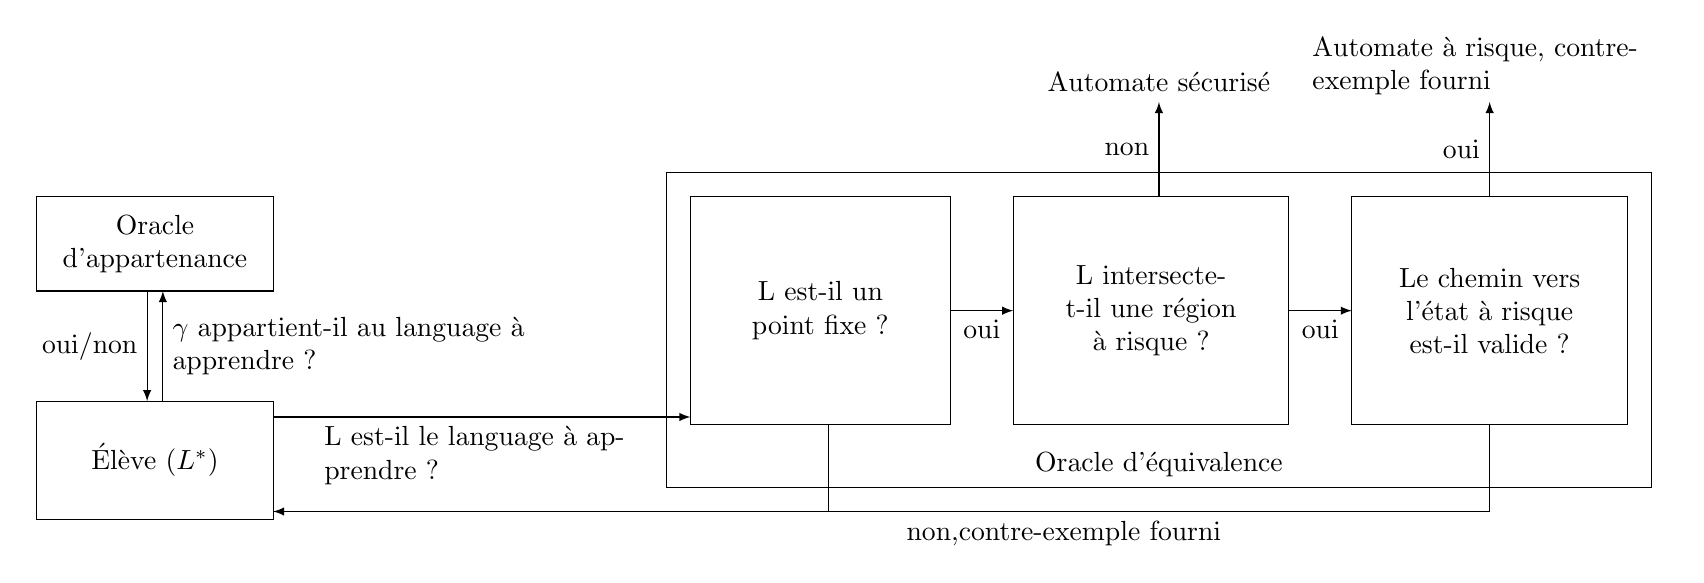
\begin{tikzpicture}
	\tikzset{>=latex}

  \draw (-3,-2.9) rectangle (0,-4.4) node[pos=.5] {Élève ($L^*$)};
  \draw (5,0) rectangle (17.5,-4);
	\draw[->] (0,-3.1) -- (5.3,-3.1) node[pos=0.5,below,text width=4cm] {L est-il le language à apprendre ?};

  \draw (-3,-0.3) rectangle (0,-1.5) node[pos=.5,text width=3cm,align=center] {Oracle\\ d'appartenance};
  \draw[->] (-1.4,-2.9) -- (-1.4,-1.5) node[pos=0.5,right,text width=5cm] {$\gamma$ appartient-il au language à apprendre ?};
  \draw[<-] (-1.6,-2.9) -- (-1.6,-1.5) node[pos=0.5,left] {oui/non};

  \node[draw=none] at (11.25, -3.7) {Oracle d'équivalence};

  \draw (5.3, -0.3) rectangle (8.6, -3.2) node[pos=0.5,text width=3cm,align=center] {L est-il un point fixe ?};
  \draw (9.4, -0.3) rectangle (12.9, -3.2) node[pos=0.5,text width=3cm,align=center] {L intersecte-t-il une région à risque ?};
  \draw (13.7, -0.3) rectangle (17.2, -3.2) node[pos=0.5,text width=3cm,align=center] {Le chemin vers l'état à risque est-il valide ?};

  \draw[->] (8.6, -1.75) -- (9.4,-1.75) node[pos=0.5,below] {oui};
  \draw[->] (12.9, -1.75) -- (13.7,-1.75) node[pos=0.5,below] {oui};
  \draw[->] (15.45, -4.3) -- (0, -4.3) node[pos=0.35,below] {non,contre-exemple fourni};
  \draw[-] (7.05, -3.2) -- (7.05, -4.3);
  \draw[-] (15.45, -3.2) -- (15.45, -4.3);

	\draw[->] (11.25,-0.3) -- (11.25,0.9)node[pos=0.5,left] {non};
	\draw[->] (15.45,-0.3) -- (15.45,0.9)node[pos=0.5,left] {oui};

	\node[draw=none] at (11.25, 1.15) {Automate sécurisé};
	\node[draw=none,text width=4.5cm] at (15.45, 1.36) {Automate à risque, contre-exemple fourni};


\end{tikzpicture}
}
\caption{Vue schématique de l'algorithme d'Angluin pour LeVer\cite{Vardhan04}}\label{fig:lever}
\end{figure}


\emph{LeVer} est le nom de cette technique. En particulier, on peut noter sur ce schéma que l'oracle d'équivalence peut non seulement répondre oui ou non mais également interrompre l'apprentissage s'il est possible de se prononcer sur la sûreté d'un automate à files $F$. Pour rappel, $L(F)$ n'est pas régulier en général. Pouvoir se prononcer sur la sûreté de $F$ étant possible, il n'est ni utile ni forcémment possible de continuer à appliquer $L^*$ pour obtenir une meilleure approximation $L$ du langage de trace de $F$. 

\section{Trace annotée}\label{trace}Cette section s'intéresse aux langages qui peuvent être associés à un automate. La section \ref{ss:trace} défini le langage de trace d'un automate. Celui-ci n'est pas nécessairement régulier. Les sections suivantes s'appuyent sur \cite{Vardhan04} pour proposer un langage régulier qui représente ce langage de trace.


% ██       █████  ███    ██  ██████
% ██      ██   ██ ████   ██ ██
% ██      ███████ ██ ██  ██ ██   ███
% ██      ██   ██ ██  ██ ██ ██    ██
% ███████ ██   ██ ██   ████  ██████

\subsection{Langage tracé}\label{ss:trace}

Une façon de définir un langage à partir d'un automate FIFO est de s'intéresser aux noms des transitions suivies lors de l'exécution. Cette section défini les éléments permettant d'arriver à la construction d'un tel langage.

Dans un système de transitions \tsys, la fonction de transition $\rightarrow:S\times\Theta\rightarrow S$ permet de définir le passage d'un état à un autre.

La \emph{fonction de transition étendue} $\xrightarrow{*}$ est la fermeture transitive et réflexive de $\rightarrow$.

Pour une suite de noms de transitions $\sigma=\theta_1\theta_2 ...\theta_n\in\Theta^*$, on note $(p,w)\xrightarrow{\sigma}(q,w')$ si il existe des états $(p_1,w_1)(p_2,w_2)...(p_{n-1},w_{n-1})$ tels que $(p,w)\xrightarrow{\theta_1}(p_1,w_1)\xrightarrow{\theta_2}...\xrightarrow{\theta_{n-1}}(p_{n-1},w_{n-1})\xrightarrow{\theta_n}(q,w')$. Dans ce cas, $\sigma$ est une \emph{trace de chemin}.

\begin{definition} Soit un automate FIFO $F$ et l'état initial $s_0=(q_0, \epsilon^C)$. Celui-ci est le couple état de contrôle initial $q_0$ ainsi que des mots $w[c]=\epsilon$ pour tout canal $c\in C$.

  Le \emph{langage de trace} d'un automate $F$ est

  $$
  L(F)=\{\sigma\in\Theta^*|\exists s=(p,w) \text{ tel quel } s_0\xrightarrow{\sigma}s\}
  $$
\end{definition}

\begin{example}
  Considérons l'automate FIFO $F$ de la figure \ref{fig:fifo1}.

  Pour celui-ci, $\sigma=\theta_1\theta_4\theta_7$ n'est pas un chemin. En effet,
  $$
  (q_0,[\epsilon,\epsilon])\xrightarrow{\theta_1}(q_1,[0,\epsilon])\xrightarrow{\theta_4}(q_3,[\epsilon,\epsilon])
  $$

  Mais, il n'existe pas d'état $s$ tel que $(q_3,[\epsilon,\epsilon])\xrightarrow{\theta_7}s$. En effet, pour appliquer cette transition, il aurait fallu que le canal $b$ contienne un symbole $0$. Ce n'est pas le cas.


  Par contre, $\sigma=\theta_2\theta_5\theta_5\theta_6\theta_7\theta_1\theta_4\theta_7$ est un chemin dans $F$ :
  \begin{equation*}
    \begin{gathered}
      (q_0,[\epsilon,\epsilon])\xrightarrow{\theta_2}
      (q_0,[1,\epsilon])\xrightarrow{\theta_5}
      (q_0,[1,0])\xrightarrow{\theta_5}
      (q_0,[1,00])\xrightarrow{\theta_6}
      (q_0,[\epsilon,00])\xrightarrow{\theta_7}\\
      (q_0,[\epsilon,0])\xrightarrow{\theta_1}
      (q_0,[0,0])\xrightarrow{\theta_4}
      (q_0,[\epsilon,0])\xrightarrow{\theta_7}
      (q_0,[\epsilon,\epsilon])
    \end{gathered}
  \end{equation*}

  On a bien un état $s$ (ici $s=(q_0,[\epsilon,\epsilon])=s_0$) tel que $s_0\xrightarrow{\sigma}s$.

\end{example}

  % ████████ ██   ██ ███████ ████████  █████
  %    ██    ██   ██ ██         ██    ██   ██
  %    ██    ███████ █████      ██    ███████
  %    ██    ██   ██ ██         ██    ██   ██
  %    ██    ██   ██ ███████    ██    ██   ██



\subsection{Alphabet d'annotation}

Le langage de trace n'est pas nécessairement régulier. Pour permettre l'apprentissage par l'algorithme d'Angluin, il faut en construire un qui est régulier et qui permette de reconstruire le langage de trace. Pour ce faire, ce nouveau langage devrait pouvoir représenter tout état atteignable ainsi qu'un ou plusieurs chemins ou mots témoins permettant d'atteindre ceux-ci.

Pour ce faire, pour chaque nom de transition correspondant à une action d'envoi, un \emph{co-nom} est défini :
$$
\bar{\Theta}=\{\bar{\theta}|\theta\in\Theta\wedge\exists p,q \in Q, c\in C, a\in\Sigma,\text{tels que } \delta(\theta)=(p,c!a,q)\}
$$

De plus, un \emph{symbole de contrôle} est créé pour chaque état de contrôle : $T_Q = \{t_q | q\in Q\}$.

En combinant les noms de transitions, les co-noms et les symboles de contrôlé, un nouvel alphabet peut-être défini, l'\emph{alphabet d'annotation} : $\Phi=(\Theta-\Theta_r)\bigcup\bar{\Theta}\bigcup T_Q$.

Avec $\Theta_r=\{\theta|\theta\in\Theta\wedge\exists p,q \in Q, c\in C, a\in\Sigma,\text{tels que } \delta(\theta)=(p,c?a,q)\}$, similaire à $\bar{\Theta}$ mais avec un nom pour chaque transition pour les actions de réception.


\subsection{Trace annotée}


Soit $\mathcal{A}:\Theta^*\rightarrow\Phi^*$ une fonction associant une \emph{trace annotée} à une trace d'automate. Soit une séquence de transitions $\sigma\in\Theta^*$. Pour chaque transition $\theta_{ri}\in\sigma$ associée à une action de réception,


\begin{algorithm}[H]
  	\begin{algorithmic}[1]
    \REQUIRE une suite de noms de transitions $\sigma\in\Theta^*$
		\ENSURE une trace annotée $\gamma\in\Phi^*$ représentant $\sigma$

    \STATE $\gamma\leftarrow\epsilon$
    \FORALL {transition $\theta\in\sigma$}
      \IF {$\theta$ correspond à une action de réception}
        \STATE trouver $\theta_s\in\Theta$ correspondant à une action d'envoi antécédant dans $\sigma$ tel que les actions s'appliquent sur le même canal et le même symbole
        \STATE remplacer $\theta_s$ par $\bar{\theta_s}\in\bar{\Theta}$
      \ELSIF {$\theta$ correspond à une action d'envoi}
        \STATE ah
      \ENDIF
    \ENDFOR

		\RETURN Vrai
	\end{algorithmic}
	\caption{$\mathcal{A}:\Theta^*\rightarrow\Phi^*$}\label{alg:A}
\end{algorithm}








Intuitivement, le \emph{langage de trace annotée} est composé d'éléments de \barTheta désignant des actions d'envoi qui n'ont plus d'impact (une action de réception pour le même symbole dans le même canal a eu lieu), suivie d'actions d'envoi impactant encore l'exécution de l'automate. Pour respecter la propriété attendue de donner un état et son témoin, le symbole de contrôle de l'état de contrôle obtenu par la liste de symboles est ajouté à la fin.
Séquence de transitions $l$ pas égal à $\sigma$ : sigma montre les états et est d'office valide !
Wait. Si $l\in L(F)$ mon argument s'évapore.

\section{Appartenance}\label{mem}\begin{algo}[Appartenance à $AL(F)$]\label{alg:membership}
  \begin{algorithmic}[1]
    \REQUIRE une trace annotée $\gamma\in\Phi^*$ et un automate FIFO \fifo
    \ENSURE si $\gamma\in AL(F)$ ou non
    \IF {$t$ est mal formaté}
      \RETURN faux
    \ENDIF
    \STATE candidats $\leftarrow\{(q_0,\epsilon^c)\}$
    \FORALL {symbole $\phi \in t$}
      \IF {$\phi \in T_Q$}
        \STATE \COMMENT {Fin du mot}
        \FORALL {$(q,w)\in$ candidats}
          \IF {$\phi$ est un $t_q$ correspondant à $q$}
            \RETURN vrai
          \ENDIF
        \ENDFOR
        \RETURN faux
      \ELSE
        \STATE \COMMENT{Exécution de l'automate sur une étape}
        \STATE nouveau $\leftarrow\emptyset$
        \STATE extension $\leftarrow\emptyset$
        \FORALL {$(q,w)\in$ candidats}
          \STATE $\phi'\leftarrow\phi$ sans l'éventuelle barre
          \STATE \COMMENT {Permet de rejeter les chemins incorrects sans effectuer l'exécution complète}
          \STATE ajouter $\delta(\phi', (q,w))$ à extension si $\delta$ est définie pour ces valeurs
        \ENDFOR
        \STATE \COMMENT {Complète avec les actions de réception possibles}
        \WHILE {extension est non vide}
          \STATE \COMMENT {Créer les différents cas de consommation des canaux}
          \STATE prendre un élément $(q,w)\in$extension
          \FORALL {canal non-nul $c$ de $w$ commençant par un symbole $s$}
            \IF {$\exists\theta$ correspondant à l'action $c?s$ sortant de $q$}
              \STATE \COMMENT {Comme une extension est elle-même étendue, on a récursivement les cas avec plusieurs réceptions bout à bout jusqu'à vider un canal}
              \STATE ajouter $\delta(\theta, (q,w))$ à extension
            \ENDIF
          \ENDFOR
          \STATE ajouter $(q,w)$ à nouveaux
          \STATE retirer $(q,w)$ d'extension
        \ENDWHILE
        \STATE candidats $\leftarrow$ nouveaux
      \ENDIF
    \ENDFOR
  \end{algorithmic}
\end{algo}

\section{Équivalence}\label{eq}Lorsqu'un langage régulier $L$, représenté par un automate $A_O$ tel que $L(A_O)=L$, est donné à l'oracle d'équivalence, il doit se prononcer sur $L=AL(F)$. Cependant, il ne possède pas d'automate pour $AL(F)$ qui est justement le langage recherché. Il doit alors se prononcer sur l'égalité en se basant uniquement sur $F$.

Comme expliqué dans l'introduction du chapitre, c'est impossible de façon générale. Cependant, en supposant que $AL(F)$ est régulier, il est possible de contourner le problème pour répondre à la question de sécurité.

Contrairement à la version originale de l'algorithme d'Angluin qui a deux possibilités (équivalence ou contre-exemple), celle-ci en a trois. L'oracle peut répondre soit que $AL(F)$ est sécurisé, soit qu'il ne l'est pas, soit que $L$ est différent de $AL(F)$ avec un contre-exemple.


\subsection{$L$ est-il un point fixe de $\mathcal{F}$ ?}

Cette question se base sur le théorème \ref{thm:fl} et en particulier du fait que $AL(F)$ est un point fixe. Il n'est pas possible de prouver que $L=AL(F)$ mais il est possible de montrer que $L\neq AL(F)$ en montrant que $L$ n'est pas un point fixe.

Une façon de montrer que $L\neq AL(F)$, est d'énoncer un seul élément dans $L\bigcup AL(F)-L\bigcap AL(F)=$\alfx l'union exclusive des deux ensembles. Pour rappel, $AL(F)$ est un langage contenant l'ensemble des traces valides pour l'automate à files $F$.

En comparant \fl avec $L$ pour vérifier si $L$ est un point fixe de $\mathcal{F}$, plusieurs situations peuvent apparaître :

\begin{itemize}
  \item $\mathcal{F}(L)-L\neq\emptyset$. Considérons un mot $w\in\mathcal{F}(L)-L$ et montrons que $w\in$\alfx.
  \begin{itemize}
    \item Si $w=t_{q_0}$, c'est que $t_{q_0}\notin L$. Pourtant, par définition, $t_{q_0}\in AL(F)$. Dès lors, $w\in$\alfx
    \item Sinon, si $w$ est une annotation correctement formatée, c'est que $L$ n'est pas un point fixe de $\mathcal{F}$. Dès lors, $w$ suffit à démontrer que $AL(F)\neq L$.
    \item Sinon, $w$ n'est pas une annotation correctement formatée. $w$ faisant partie de \fl, cela signifie qu'il doit exister un mot $w'\in L$ tel que $w=Post(w')$. Ce $w'$ ne peut pas être une annotation valide : cela impliquerait que $w$ l'est également ce qui est posé comme faux ici. Comme $w'$ n'est pas une annotation valide pour $F$, $w'\notin AL(F)$. Comme $w'\in L$, naturellement $w'\in$\alfx.
  \end{itemize}
  \item $\mathcal{F}(L)\subsetneq L$. Dans ce cas, utilisons la notion de point préfixe. Un ensemble $Z$ est un \emph{point préfixe} d'une fonction $\mathcal{F}$ s'il réduit par son application : $\mathcal{F}$ ($\mathcal{F}(Z)\subseteq Z$). Selon cette définition, $L$ est un point préfixe de $\mathcal{F}$.
  En appliquant $\mathcal{F}$ des deux côtés, ce qui préserve l'inclusion car $\mathcal{F}$ est monotone, on obtient $\mathcal{F}(\mathcal{F}(L))\subsetneq\mathcal{F}(L)$.

  Donc, $\mathcal{F}(L)$ est également un point préfixe. Soit $w\in L-\mathcal{F}(L)$. Comme $w$ n'est pas dans l'intersection de ces deux point préfixes, il ne fait pas partie du point fixe minimum $AL(F)$. En effet, selon la théorie des points fixes de Knaster-Tarski (annexe \ref{app:tarski}), un point fixe minimal est également l'intersection de tous les points préfixes de $\mathcal{F}$.

  \item \fl=$L$. Cela signifie que $L$ est un point fixe de $\mathcal{F}$. Cela signifie qu'il n'est pas possible de prouver que $L\neq AL(F)$ et infirmant cette propriété. Cela ne signifie par pour autant que $L=AL(F)$.

  Ce pourrait très bien être un autre point fixe contenant $AL(F)$ ou un autre ensemble contenant une trace annotée menant à un état qui n'est pas sûr. Pour tenter de continuer à chercher un contre-exemple ou tester la sûreté, il faut poser d'autres questions.

\end{itemize}



\subsection*{$L$ intersecte-t-il avec une région à risque ?}

En visualisant $L$ comme étant un super-ensemble de $AL(F)$ et la région à risque comme un ensemble, il est possible de se représenter les différentes situations envisageables.

\begin{figure}[H]

  \colorlet{circle edge}{black}
  \colorlet{circle area}{blue!20}
  \colorlet{circle darker}{blue!40}
  \tikzset{filled/.style={fill=circle area, draw=circle edge},
    outline/.style={draw=circle edge}}

  \def\circleL{ (0,0) circle (1.5cm) node[right=0.8cm]  {$L$}}
  \def\circleAL{(-0.15,-0.3) circle (1cm) node {$AL(F)$}}

 \centering
 \begin{subfigure}{0.33\textwidth}
  \centering
  \def\circleUS{(0,2.8) circle (1cm) node[text width=1.5cm,align=center]  {Région à risque}}
  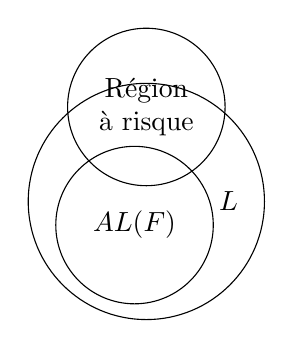
\begin{tikzpicture}
   \draw[outline]\circleL;
   \draw[outline]\circleAL;
   \draw[outline]\circleUS;
  \end{tikzpicture}
  \caption{Pas d'intersection}
 \end{subfigure}%
 \begin{subfigure}{0.33\textwidth}
  \centering
  \def\circleUS{(0,2.2) circle (1cm) node[text width=1.5cm,align=center]  {Région à risque}}
  \vspace{0.6cm}
  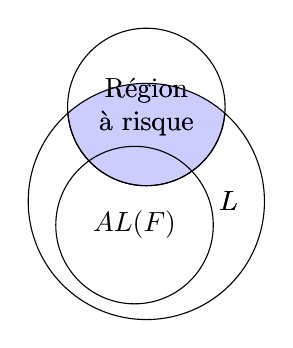
\begin{tikzpicture}
    \begin{scope}
        \clip \circleL;
        \fill[filled] \circleUS;
    \end{scope}
    \draw[outline]\circleL;
    \draw[outline]\circleAL;
    \draw[outline]\circleUS;
  \end{tikzpicture}
  \caption{Intersection avec $L$ seulement}
 \end{subfigure}
 \begin{subfigure}{0.33\textwidth}
   \centering
   \def\circleUS{(0,1.2) circle (1cm) node[text width=1.5cm,align=center]  {Région à risque}}
   \vspace{1.6cm}
   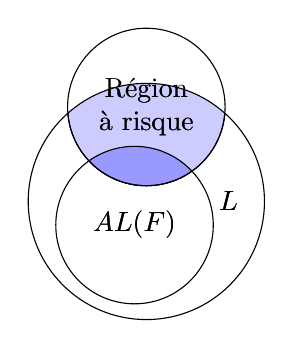
\begin{tikzpicture}
     \begin{scope}
         \clip \circleL;
         \fill[filled] \circleUS;
     \end{scope}
     \begin{scope}
         \clip \circleAL;
         \fill[filled, fill=circle darker] \circleUS;
     \end{scope}
     \draw[outline]\circleL;
     \draw[outline]\circleAL;
     \draw[outline]\circleUS;
   \end{tikzpicture}
  \caption{Intersection avec $AL(F)$}
 \end{subfigure}
 \caption{$L$, $AL(F)$ et la région à risque}\label{fig:inter}
\end{figure}

Pour savoir si nous sommes dans le scénario (a), (b) ou (c) de la figure \ref{fig:inter}, deux tests sont à effectuer.

Premièrement, vérifier si $\mathcal{W}(L)$ est vide ou non. S'il est vide, nous sommes dans le scénario (a) et il est possible d'annoncer avec certitude que $F$ est sécurisé.

\subsection*{Le chemin vers l'état à risque est-il valide ?}

Si la réponse à la question précédente est oui, sommes-nous dans le scénario (b) ou (c) ?
Considérons un des éléments de $\mathcal{W}(L)$. Demandons à l'oracle d'appartenance si ce mot appartient également à $AL(F)$.

Si ce n'est pas le cas, c'est que $L\neq AL(F)$ et que l'algorithme d'Angluin peut continuer grâce au contre-exemple fourni. Ici, il peut s'agir soit d'un scénario (b) soit d'un scénario (c) puisqu'un autre mot de $\mathcal{W}(L)$ pourrait appartenir à $AL(F)$. Améliorer l'approximation d'$AL(F)$ permet justement de mieux discriminer ces deux scénarios sans devoir consulter la totalité de $\mathcal{W}(L)$.

Si par contre le mot étudié appartient aussi à $AL(F)$, on a un mot étant à la fois dans $AL(F)$ et dans la région à risque. $F$ est déclaré à risque et le mot est retourné comme contre-exemple. Il s'agit du scénario (c).

\section{Sûreté}\label{safety}Comme mentionné au début du chapitre, ce travail s'intéresse à la propriété de sécurité dans les automates à files. Contrairement aux ADFs construits dans le chapitre \ref{ch:bases}, les automates à files ont un nombre potentiellement infini d'états. Dans ces conditions, il n'est pas possible d'énumérer l'ensemble des états acceptants.

Au lieu de proposer un ensemble d'état acceptants, on va fixer une propriété. Celle-ci permet de catégoriser les états qui sont souhaitables de ceux qui ne le sont pas. Par la suite, la section \ref{ss:tracesafety} propose une technique permettant de calculer l'ensemble des états indésirables à partir d'une trace annotée.


\subsection{Définitions}
Dans un automate à files \fifo, chaque état de contrôle $q\in Q$ est associé à un union finie de langage réguliers pour chacun des canaux $c\in C$.


$$\bigcup_{0 \leq i \leq n_q}\Pi_{0 \leq j \leq k}U_q(i,c_j)$$

Où $U_q(i,c_j)$ est un langage régulier pour le contenu du canal $c_j$ sur l'état $q$. $n_q$ est le nombre de langages réguliers utilisés pour définir cette propriété par union.

Un état $s=(q,[w_0,w_1,\dots,w_k])$ est \emph{sécurisé} s'il n'existe pas $i,j \in \mathbb{N}$ tels que $w_j \in U_q(i,c_j)$. Si tous les états d'un automate sont sécurisé, l'automate est également \emph{sécurisé}.

Si un état n'est pas sécurisé, il est \emph{à risque}. S'il existe au moins un état à risque dans un automate, celui-ci est \emph{à risque}.



\subsection{Traces annotées menant à des états à risques}\label{ss:tracesafety}

Soit la fonction $h_c:\Phi^*\rightarrow\Sigma^*$ qui, pour un trace annotée donnée, ne retourne que les messages envoyés mais non réceptionnés sur le canal $c$.

$h_c$ est l'unique homomorphisme qui étend la fonction suivante de $\Phi$ à $\Phi^*$:
$$ h_c(\theta) = \left\{ \begin{array}{ll}
      m & \text{si } \theta\in\Theta\text{ et }\delta(\theta)=(p,c!m,q)\\
      \epsilon & \text{sinon}\end{array} \right. $$



Si $L=L(F)$ alors $L_q$ est l'ensemble des mots correctements formattés pour $L$.

Si il existe un état à risque $s$, alors il existe une trace $\sigma \in \Theta^*$ telle que $s_0\xrightarrow{\sigma}s$ où $s_0$ est l'état initial. Si les transitions dénotant des actions d'envoi et de réception d'un même symbole sur un même canal sont enlevées par paires, il ne reste que les transitions participant au contenu final des différents canaux de $s$. Par définition de $h_c$, pour chaque contenu $w[c_j]$ de chaque canal $c_j$, $w[c_j]=h_{cj}(\mathcal{A}(\sigma))$. Dès lors, pour que $s$ soit atteignable, il faut qu'il existe une trace annotée $\gamma \in AL(F)$ telle que $s=(q_\gamma, [h_{c0}(\gamma),h_{c1}(\gamma),\dots,h_{ck}(\gamma)])$ où $q_\gamma$ est l'état de contrôle désigné par le symbole de contrôle à la fin de $\gamma$.

Soit la fonction $h^{-1}_{c}:\Sigma^*\rightarrow\Phi^*$ l'homomorphisme inverse de $h_c$. C'est-à-dire $h^{-1}_{cj}(U_q(i,c_j))$ retourne des traces annotées correspondant au contenu d'un canal. Dans ce cas particulier, un des langages réguliers servant à définir la propriété de sécurité. Comme un plusieurs traces annotées peuvent correspondre au même contenu de canaux par $h_c$, un contenu de canal peut correspondre à plusieurs traces annotées via $h^{-1}_c$.

En calculant cette fonction pour l'ensemble des états, canaux et langages réguliers définissant la sécurité de $F$ et en s'assurant que ces traces sont correctement formatées, on obtient un ensemble de traces menant à des états à risque-.

Cet ensemble est décrit mathématiquement par $\mathcal{W}(L)$ :
$$
\mathcal{W}(L)=\bigcup_{q\in Q}\big(\bigcup_{0\leq i\leq n_q}\big(\bigcap_{0\leq j \leq k}h_{c_j}^{-1}(U_q(i,c_j))\big)\big)
$$

%\section{Algorithme}\label{lever}Dans les chapitres précédants, les bases théoriques sur les automates et languages ont été introduites. Celles-ci ont été suivies de concepts plus étroitement liés à LeVer tels que les automates à files, les traces, traces annotées et languages associés. Un dernier élément présenté dans la section \ref{sec:unsafe} est la sécurité d'un état ou d'un automate.

En appliquant l'algorithme d'Angluin \cite{Angluin87} selon la méthode LeVer \cite{Vardhan04}, il est possible de se prononcer sur la sécurité pour toute une classe d'automates à files : ceux pour lesquels le language de traces annotées est régulier.

L'objectif dès lors n'est pas d'apprendre le language de l'automate à file mais le language de trace associé, et d'adapter la méthode pour répondre à la question de sécurité. En formulant les bonnes propriétés, il est également possible d'interrompre l'algorithme d'apprentissage avant terme si l'on peut se prononcer sur la sécurité de façon certaine.


\begin{figure}[H]
	\centering

	\resizebox{\textwidth}{!}{
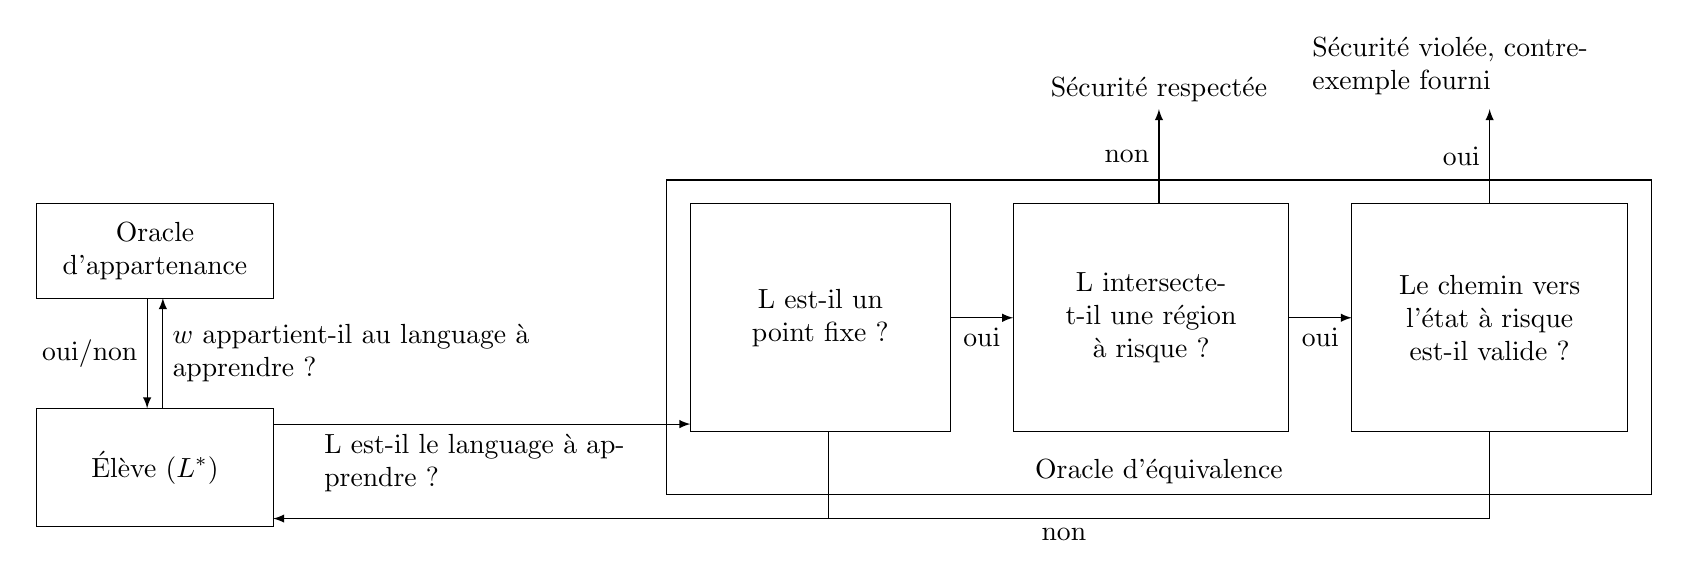
\begin{tikzpicture}
	\tikzset{>=latex}

  \draw (-3,-2.9) rectangle (0,-4.4) node[pos=.5] {Élève ($L^*$)};
  \draw (5,0) rectangle (17.5,-4);
	\draw[->] (0,-3.1) -- (5.3,-3.1) node[pos=0.5,below,text width=4cm] {L est-il le language à apprendre ?};

  \draw (-3,-0.3) rectangle (0,-1.5) node[pos=.5,text width=3cm,align=center] {Oracle\\ d'appartenance};
  \draw[->] (-1.4,-2.9) -- (-1.4,-1.5) node[pos=0.5,right,text width=5cm] {$w$ appartient-il au language à apprendre ?};
  \draw[<-] (-1.6,-2.9) -- (-1.6,-1.5) node[pos=0.5,left] {oui/non};

  \node[draw=none] at (11.25, -3.7) {Oracle d'équivalence};

  \draw (5.3, -0.3) rectangle (8.6, -3.2) node[pos=0.5,text width=3cm,align=center] {L est-il un point fixe ?};
  \draw (9.4, -0.3) rectangle (12.9, -3.2) node[pos=0.5,text width=3cm,align=center] {L intersecte-t-il une région à risque ?};
  \draw (13.7, -0.3) rectangle (17.2, -3.2) node[pos=0.5,text width=3cm,align=center] {Le chemin vers l'état à risque est-il valide ?};

  \draw[->] (8.6, -1.75) -- (9.4,-1.75) node[pos=0.5,below] {oui};
  \draw[->] (12.9, -1.75) -- (13.7,-1.75) node[pos=0.5,below] {oui};
  \draw[->] (15.45, -4.3) -- (0, -4.3) node[pos=0.35,below] {non};
  \draw[-] (7.05, -3.2) -- (7.05, -4.3);
  \draw[-] (15.45, -3.2) -- (15.45, -4.3);

	\draw[->] (11.25,-0.3) -- (11.25,0.9)node[pos=0.5,left] {non};
	\draw[->] (15.45,-0.3) -- (15.45,0.9)node[pos=0.5,left] {oui};

	\node[draw=none] at (11.25, 1.15) {Sécurité respectée};
	\node[draw=none,text width=4.5cm] at (15.45, 1.45) {Sécurité violée, contre-exemple fourni};


\end{tikzpicture}
}
\caption{Vue schématique de l'algorithme d'Angluin pour LeVer\cite{Vardhan04}}

\end{figure}


\todo{Ce chapitre décrit le fonctionnement de LeVer en se basant sur tout le reste. Concrètement, il s'agit d'une reformulation de l'algorithme d'Angluin pour les automates FIFO selon la méthode de Vardhan}

\todo{Cette section explique le but recherché, son importance et la structure du chapitre}

